% XeLaTeX can use any Mac OS X font. See the setromanfont command below.
% Input to XeLaTeX is full Unicode, so Unicode characters can be typed directly into the source.

% The next lines tell TeXShop to typeset with xelatex, and to open and save the source with Unicode encoding.

%!TEX TS-program = xelatex
%!TEX encoding = UTF-8 Unicode

\documentclass[UTF8]{ctexart}
\usepackage{geometry}                % See geometry.pdf to learn the layout options. There are lots.
\geometry{letterpaper}                   % ... or a4paper or a5paper or ...
%\geometry{landscape}                % Activate for for rotated page geometry
%\usepackage[parfill]{parskip}    % Activate to begin paragraphs with an empty line rather than an indent
\usepackage{graphicx}
\usepackage{amssymb}
\usepackage{enumerate}
\usepackage{booktabs}
\usepackage{multirow}
\usepackage{float}
% Will Robertson's fontspec.sty can be used to simplify font choices.
% To experiment, open /Applications/Font Book to examine the fonts provided on Mac OS X,
% and change "Hoefler Text" to any of these choices.

\usepackage{fontspec,xltxtra,xunicode}
\defaultfontfeatures{Mapping=tex-text}
\setromanfont[Mapping=tex-text]{Hoefler Text}
\setsansfont[Scale=MatchLowercase,Mapping=tex-text]{Gill Sans}
\setmonofont[Scale=MatchLowercase]{Andale Mono}

\title{\Huge \textbf{软件工程项目文档}  \\
\large ~~~~~~~ ———— “鲜活”社团管理平台
 ~\\ ~\\ ~\\ ~\\ ~\\ ~\\ ~\\ ~\\ ~\\ ~\\ ~\\}
\author{
\large 指导老师:黄杰 \\
\large 1452822 洪嘉勇 \\
\large 1454093 夏陈   \\
\large 1452716 张尹嘉 \\
}
%\date{}                                           % Activate to display a given date or no date

\begin{document}
\maketitle

% For many users, the previous commands will be enough.
% If you want to directly input Unicode, add an Input Menu or Keyboard to the menu bar
% using the International Panel in System Preferences.
% Unicode must be typeset using a font containing the appropriate characters.
% Remove the comment signs below for examples.

% \newfontfamily{\A}{Geeza Pro}
% \newfontfamily{\H}[Scale=0.9]{Lucida Grande}
% \newfontfamily{\J}[Scale=0.85]{Osaka}

% Here are some multilingual Unicode fonts: this is Arabic text: {\A السلام عليكم}, this is Hebrew: {\H שלום},
% and here's some Japanese: {\J 今日は}.

\newpage
\tableofcontents
\newpage

\section{引言}
\subsection{背景}
近年来互联网、物联网等发展迅猛,高校校园在这波潮流中可以说是弄潮儿,很多互联网创新平台都在高校中运行得非常稳健。学校也正利用着这股潮流做着相应的改变,校园的管理系统正在渐渐地完善,比如图书馆的预览室已经可以在网上平台预约、校车也可以在网上抢票,但是跟学生们的课余生活最为密切的社团生活似乎并没有纳入学校网络化的考虑范围中。与此同时,我们的社团的活动也开始缺乏新意,社团的团长们缺乏好的点子,而在互联网+的时代下,去创建这样一二个信息共享的渠道是相对容易的,我们渴望在这个时代背景下为同济大学师生创建一个社团管理平台和社团活动信息共享平台,我们将其命名为“鲜活”。
\paragraph{同济大学社团发展现状}
就目前同济大学校园而言,大多数关于社团的操作都非常地繁琐,通信的时间成本和经济成本都非常高,很多社团的发展因为制度问题而变得不健康。体现在以下方面:

\begin{enumerate}[1)]
\item 社团审批需要递交的材料多且审批等待时间长,将导致很多新兴社团痛失很多招生机会
\item 很多社团缺少展示的平台,很多社团因此默默无闻
\item 社团自身没有统一的管理规范,社团管理比较混乱
\item 社团通信流程复杂,通知时间成本高
\item 社团申请场地和申请海报张贴的流程繁琐,等待时间长
\end{enumerate}

\paragraph{线上平台的必要性}
现行的体制使得社团发展受到遏制,一个线上统一管理社团的平台已经成为师生共同的需求。而且传统的在食堂门口发传单等宣传方式早已受到师生们的反感,也为校园环保造成一定的压力,这些事情完全可以放在线上平台上来做。师生们渴望社团是一个又鲜又活的东西,而不是一个抽象的存在,我们需要想办法加强社团的存在感。而这一切都可以通过一个线上的社团管理平台实现。

\paragraph{线上平台的可行性}
在经过背景分析和技术论证之后,我们认为线上平台的可行性很强,具体为以下几点:

\begin{enumerate}[1)]
\item 互联网已经普及
\item 师生群体中智能手机普及率接近100\%
\item 同济大学“同心云”轻应用可以成为一个很好的展示平台
\end{enumerate}

\subsection{假设和约束}
\paragraph{基本假设}本项目需要以一些基本的假定作为项目开展的基础。我们以一些普遍的认识和经验作出以下假设:

\begin{enumerate}[1)]
\item 师生都有手机并可以访问互联网
\item 可以得到学校的支持将平台的展示页面搭载于同济大学“同心云”上
\item 学校可以授权我们得到相关社团和成员的信息
\end{enumerate}

\paragraph{基本约束}
本项目需要以一些基本的约束作为项目开展的基础。我们经过讨论作出以下约束:

\begin{enumerate}[1)]
\item 为减轻服务器访问压力,平台的用户仅限于同济大学的师生,即拥有同济大学学号和工号的人群
\item 团学联老师拥有管理员权限
\item 将尊重所有用户的个人隐私,对用户的个人信息保密
\item 项目开发经费限于大学生国家创新项目经费所给的10000元
\item 项目初期将部署于阿里云服务器上作初步测试
\item 开发时限:2015年-2017年
\item 咨询推送功能将因为课设时间紧迫无法上线
\end{enumerate}

\subsection{用户的特点}
“鲜活”是一个为同济大学师生服务的社团管理和活动信息共享平台,用户主体为同济大学的师生,我们将所有用户罗列如下:

\paragraph{老师}
\subparagraph{概述}
老师是“鲜活”中具有上帝权限的管理员,老师可作为基本用户像学生一样去参加社团甚至可以创建社团,也可以接收到社团的消息推送。但是最关键的是,老师可以审核社团的申请以及社团对场地的申请,只有在老师同意的情况下,社团才可以进行之后的操作。
\subparagraph{具体可执行操作}
老师具体可执行的操作如下:
\newline
\newline
\begin{table}[H]
\centering
\caption{老师}
\begin{tabular}{ccc}
\toprule
操作& 描述\\
\midrule
\textbf{创建社团}& 老师也可以创建属于自己的社团\\
\textbf{加入某个社团}& 老师可以参加某个社团\\
\textbf{参加某个活动}&老师可以参加某个社团的某个活动\\
\textbf{同意社团的创建申请}&老师将审阅所有社团的申请并决定是不是让这个社团成立并入驻“鲜活”\\
\textbf{同意社团的场地申请}&老师将审阅社团的场地申请请求并根据场地借用记录决定是否出借场地\\
\bottomrule
\end{tabular}
\end{table}

\paragraph{社团负责人}
\subparagraph{概述}
社团负责人是“鲜活”中的核心角色,社团负责人在平台中和普通用户一样,只是因为他们申请了社团所以成为了社团负责人这样一个特殊的角色。他们作为社团的核心人物会在平台上管理他们的社团,发布他们的活动和通知,并向上级老师申请活动的场地。
\subparagraph{具体可执行操作}
社团负责人可执行的操作如下:
\newline
\newline
\begin{table}[H]
\centering
\caption{社团负责人}
\begin{tabular}{ccc}
\toprule
操作& 描述\\
\midrule
\textbf{创建社团}& 社团负责人可以向老师发出申请创建属于自己的社团\\
\textbf{加入某个社团}& 社团负责人可以参加某个社团\\
\textbf{参加某个活动}&社团负责人可以参加某个社团的某个活动\\
\textbf{查看社员}&社团负责人可以在“鲜活”中看到谁参加了自己的社团并得到他们的一些信息\\
\textbf{发布活动}&社团负责人可以在“鲜活”中发布自己社团的活动并通过平台向所有社员推送活动信息\\
\textbf{群发短信}& 社团负责人可以根据自己的需求向自己的社员群发短信\\
\textbf{评论}& 社团负责人可以评论不是自己的社团但是他可以评论任何活动\\
\bottomrule
\end{tabular}
\end{table}

\paragraph{普通学生}
\subparagraph{概述}
普通学生是“鲜活”中最基本的也是最多的用户,但即便是这样,一旦等他准备好发起了创建社团的申请并通过审核,就会成为一名社团负责人。普通学生可以加入任何社团中并参加任何社团开始的社团活动,在进入社团后可以下载社团中的资源文件。他们会接收到社团发送的通知。
\subparagraph{具体可执行操作}
普通学生可执行的操作如下:
\newline
\newline
\begin{table}[H]
\centering
\caption{普通学生}
\begin{tabular}{ccc}
\toprule
操作& 描述\\
\midrule
\textbf{创建社团}& 普通学生也可以向老师发起申请创建属于自己的社团\\
\textbf{加入某个社团}& 普通学生可以参加某个社团\\
\textbf{参加某个活动}& 普通学生可以参加某个社团的某个活动\\
\textbf{评论}& 普通学生可以评论任何社团或者任何活动\\
\bottomrule
\end{tabular}
\end{table}

\section{功能需求}
\subsection{系统范围}
\subsubsection{系统开发的意图}
旨在开发一个为同济大学师生服务的线上社团管理平台和社团活动共享平台,将社团从创建到招新到发布活动一体化。
\subsubsection{应用目标}
本系统的应用目标主要为同济大学“同心云”的轻应用和一个web端。
\paragraph{“同心云”轻应用}
本系统将在“同心云”上搭载一个轻应用与服务器相连,用户可以在同心云上查看社团的相关信息并可以进行相关操作,操作将会被同步到web端。但在轻应用上,将不具备社团负责人管理社团的功能,涉及社团更高级的操作将只能在web端登陆之后才可以操作。
\paragraph{web端}
web端将是本系统的重点,在web端我们将开放所有版块的功能,而不仅仅是轻应用上的查看和简单操作。社团负责人可以通过web端操作社团,老师可以通过web端审核各种申请。

\subsubsection{作用范围}
本系统的作用范围为同济大学校内一切拥有同济大学统一认证学号的学生和工号的老师。
\subsection{系统体系结构}
夏
\subsection{系统总体流程}
张
\subsection{需求分析}
夏
\subsubsection{功能建模}
夏
\subsubsection{数据建模}
本系统的数据模型主要概括为:实体类(Entity)、仓库类(Repository)、服务类(Service)和控制器类(Controller),本节将着重介绍实体类、仓库类和服务类,控制器类所构成的模型在数据流图中会更加形象,故在本节中略去。
以下为本系统的数据包图和全部类的汇总:
\newline
\newline
\begin{figure}
\centering
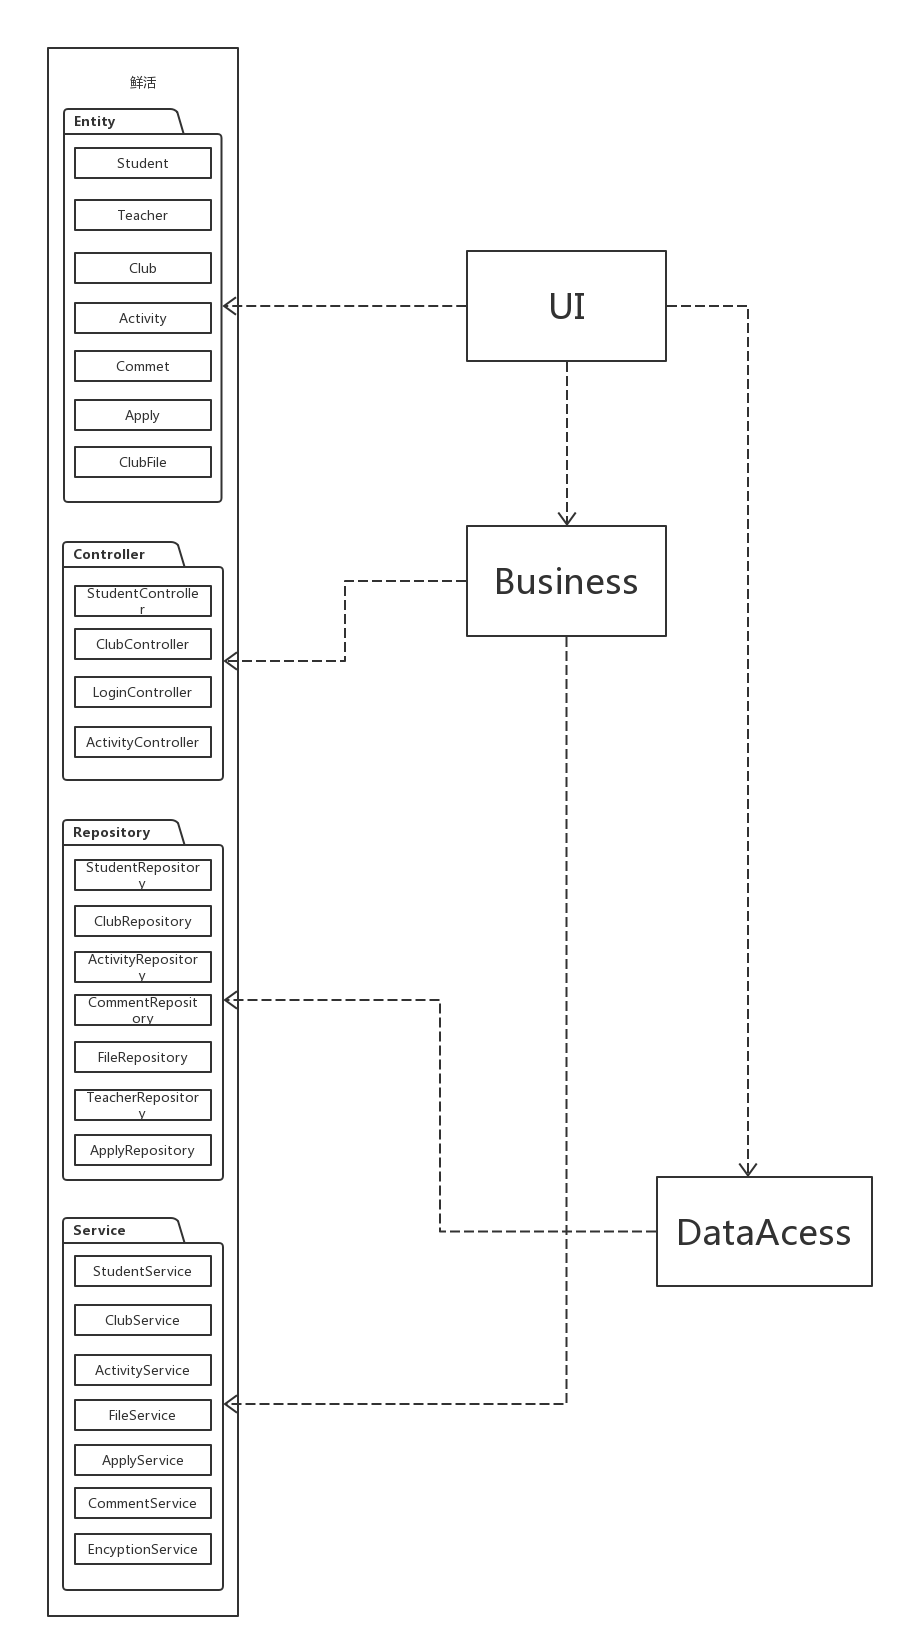
\includegraphics[width = 0.7\textwidth]{package.png}
\end{figure}

\begin{table}[H]
\centering
\caption{类汇总}
\begin{tabular}{|c|c|c|}
\hline
\multicolumn{3}{|c|}{汇总}\\
\hline
类别& 类名& 备注\\
\hline
\multirow{7}*{实体类(Entity)}
&Student& 学生\\
&Teacher&老师\\
&Club&社团\\
&Activity&活动\\
&Apply&申请\\
&Comment&评论\\
&ClubFile&社团资源文件\\
\hline
\multirow{7}*{仓库类(repository)}
&StudentRepository&学生库\\
&TeacherRepository&老师库\\
&ClubRepository&社团库\\
&ActivityRepository&活动库\\
&ApplyRepository&请求库\\
&CommentRepository&评论库\\
&clubFileRepository&社团文件资源库\\
\hline
\multirow{7}*{仓库类(repository)}
&StudentService&学生库接口\\
&TeacherService&老师库接口\\
&ClubService&社团库接口\\
&ActivityService&活动库接口\\
&ApplyService&请求库接口\\
&CommentService&评论库接口\\
&clubFileService&社团文件资源库接口\\
\hline
\end{tabular}
\end{table}

\paragraph{ER关系图}
本系统的数据库ER关系图如下:
\newline
\begin{figure}[H]
\centering
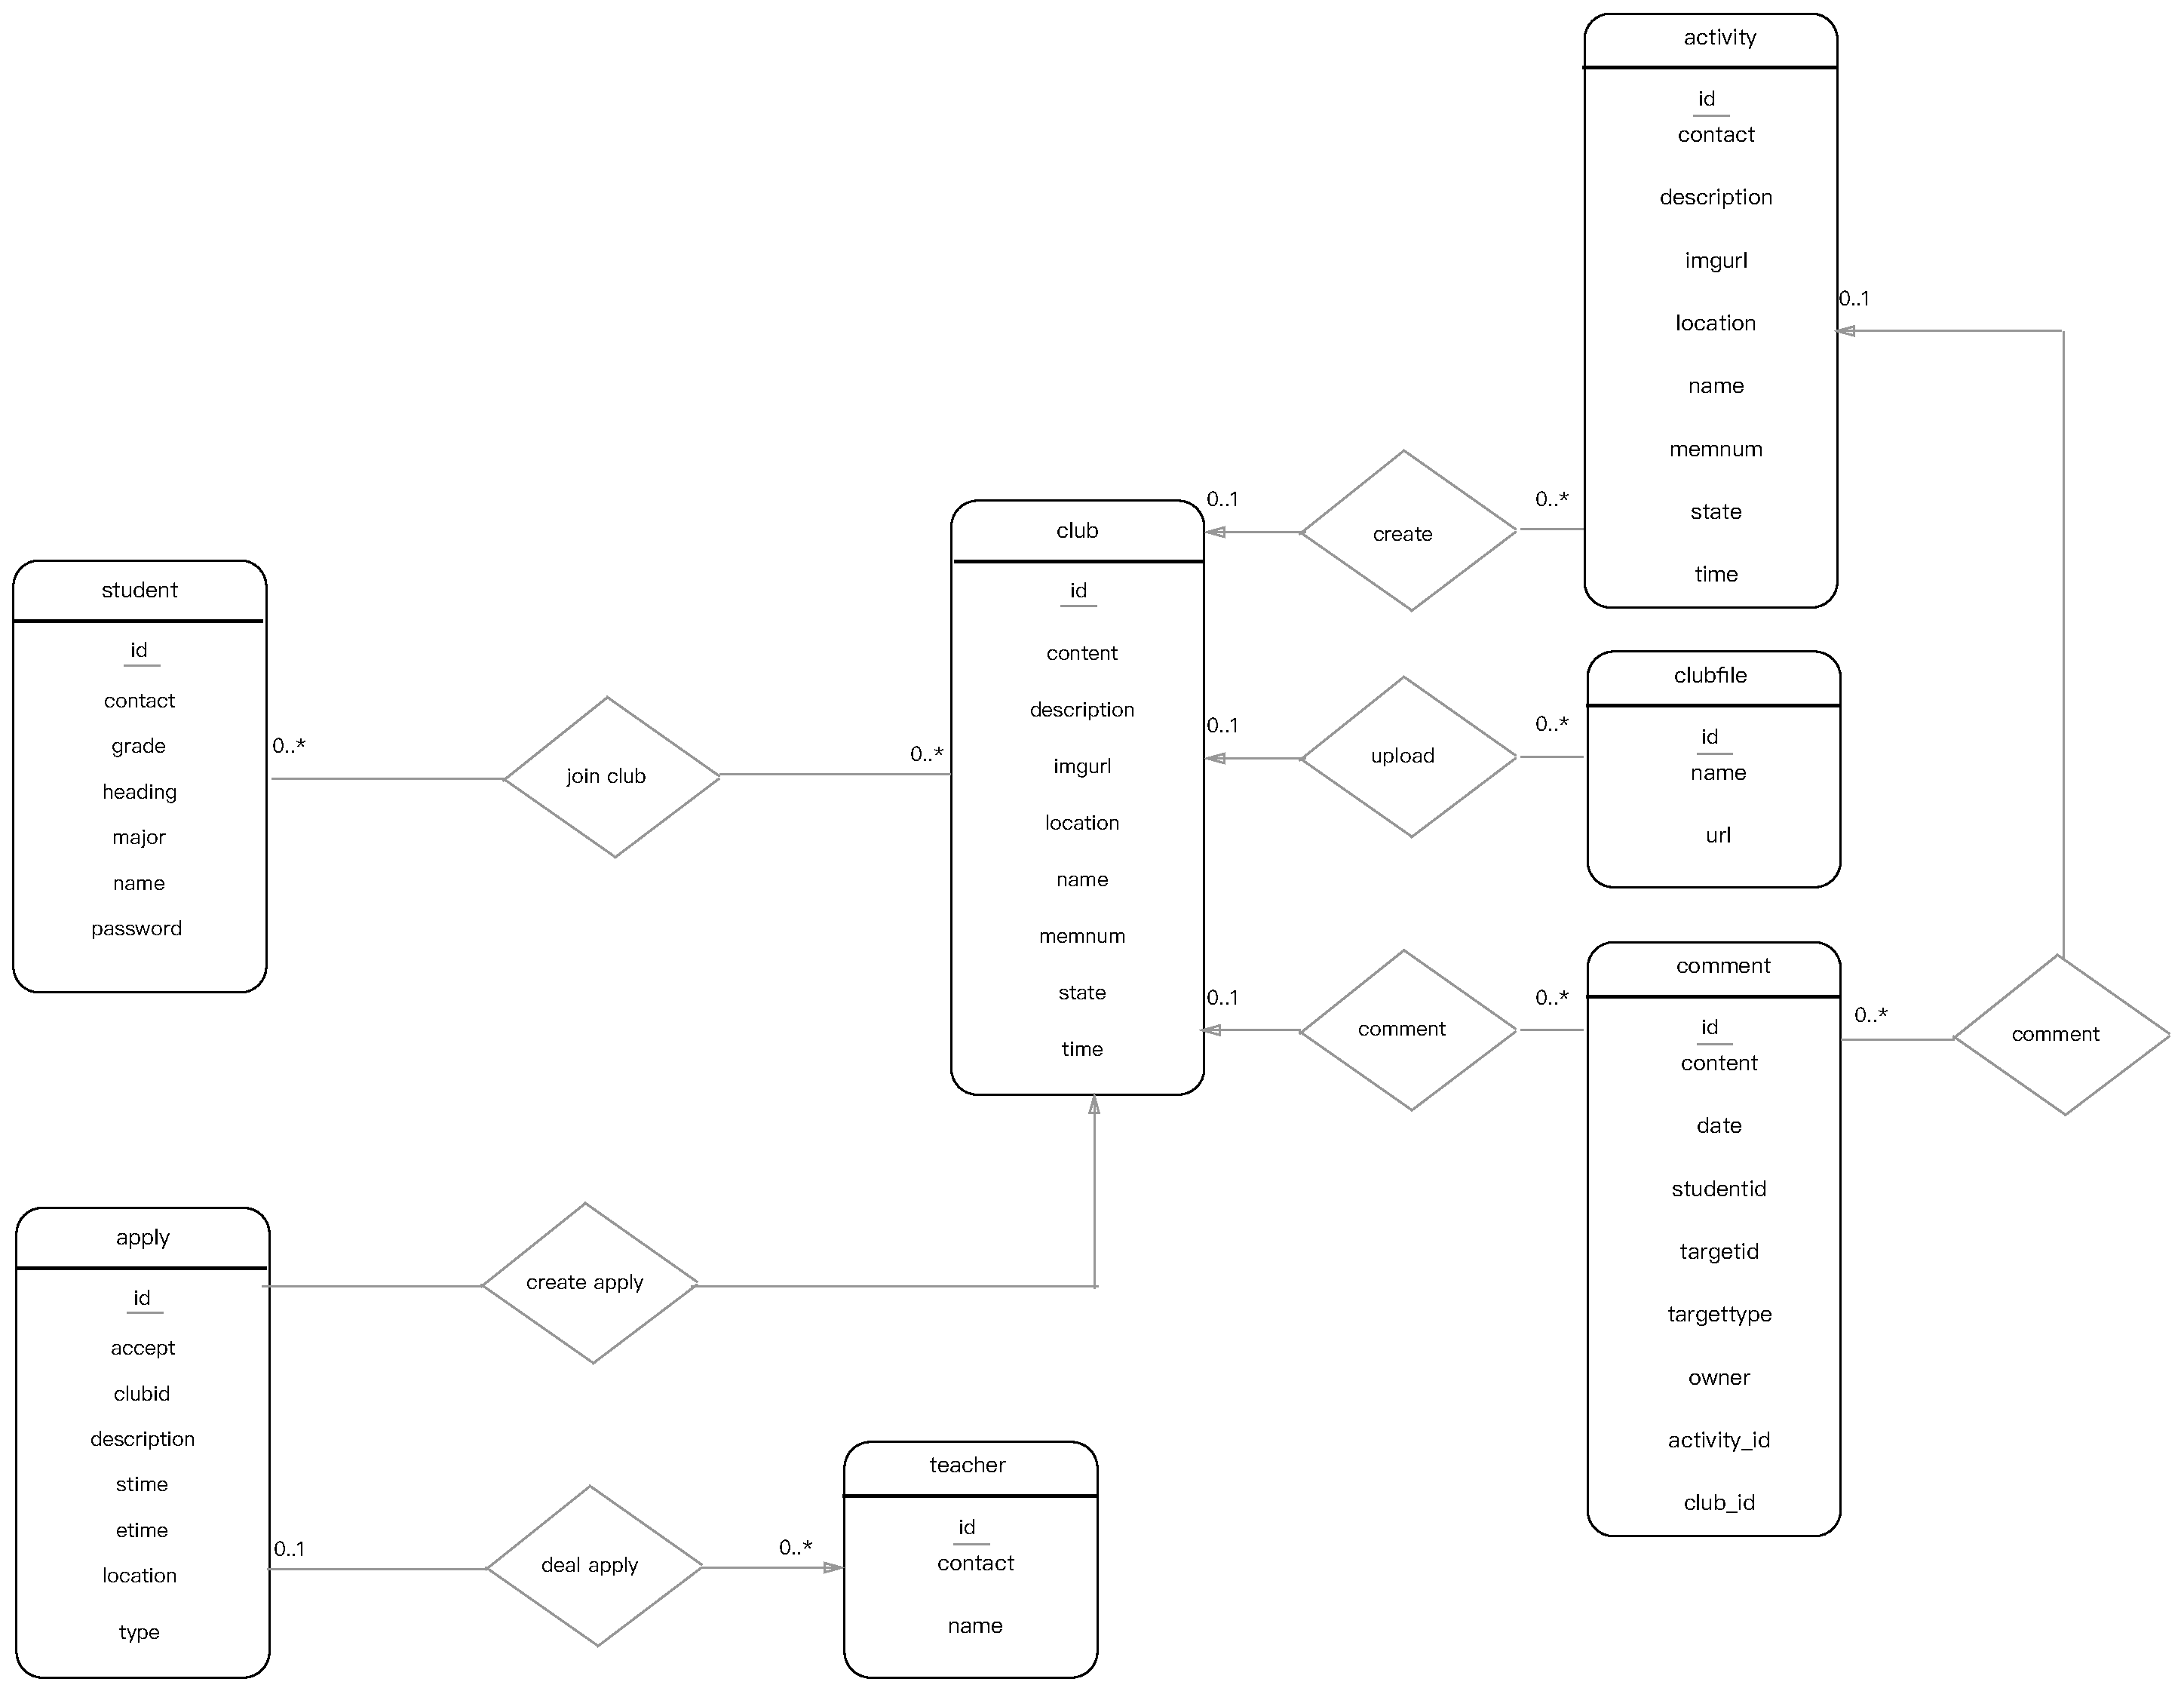
\includegraphics[width = 1.0\textwidth]{er.eps}
\end{figure}

\subparagraph{student \& club}
如下图所示,student和club以join club关系集维系,二者为多对多的关系,student申请加入club之后二者就相互关联
\newline
\begin{figure}[H]
\centering
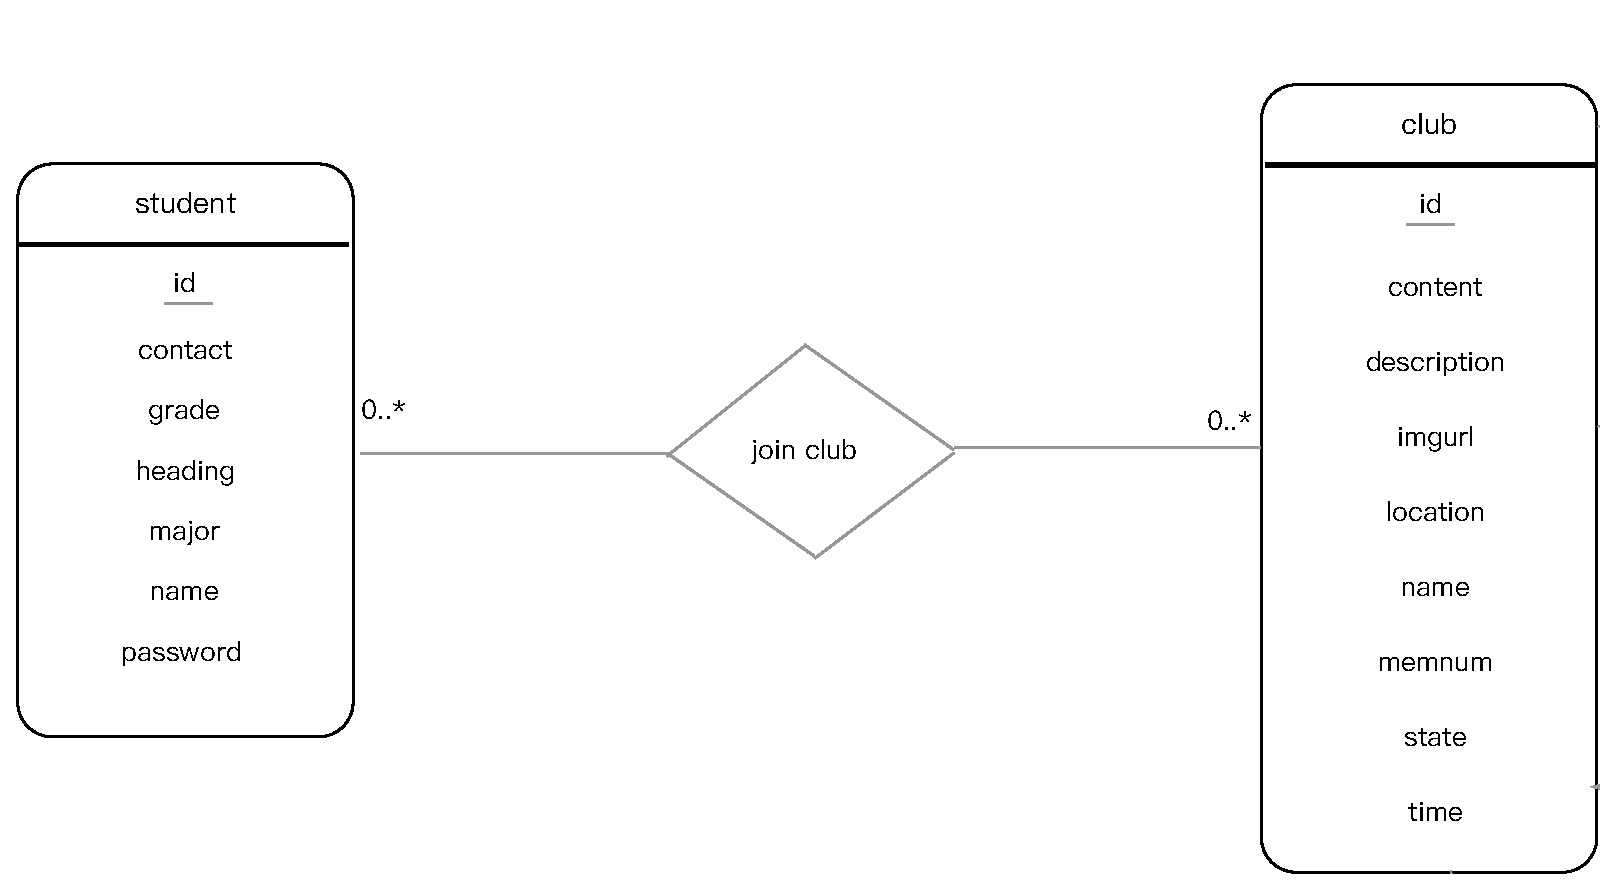
\includegraphics[width = 0.8\textwidth]{student-club-er.eps}
\end{figure}

\subparagraph{club \& activity \& clubFile \& comment}
如下图所示,club跟activity、clubFile、comment向关联。club与activity为一对多的关系,二者以create关系集维系,club可以创建很多个activity;club与clubFile也是一对多的关系,二者以upload关系集相维系,一个club可以拥有多个clubFile;club与comment也为一对多的关系,二者以comment关系集相维系,一个club可以对应多个comment。
\newline
\begin{figure}[H]
\centering
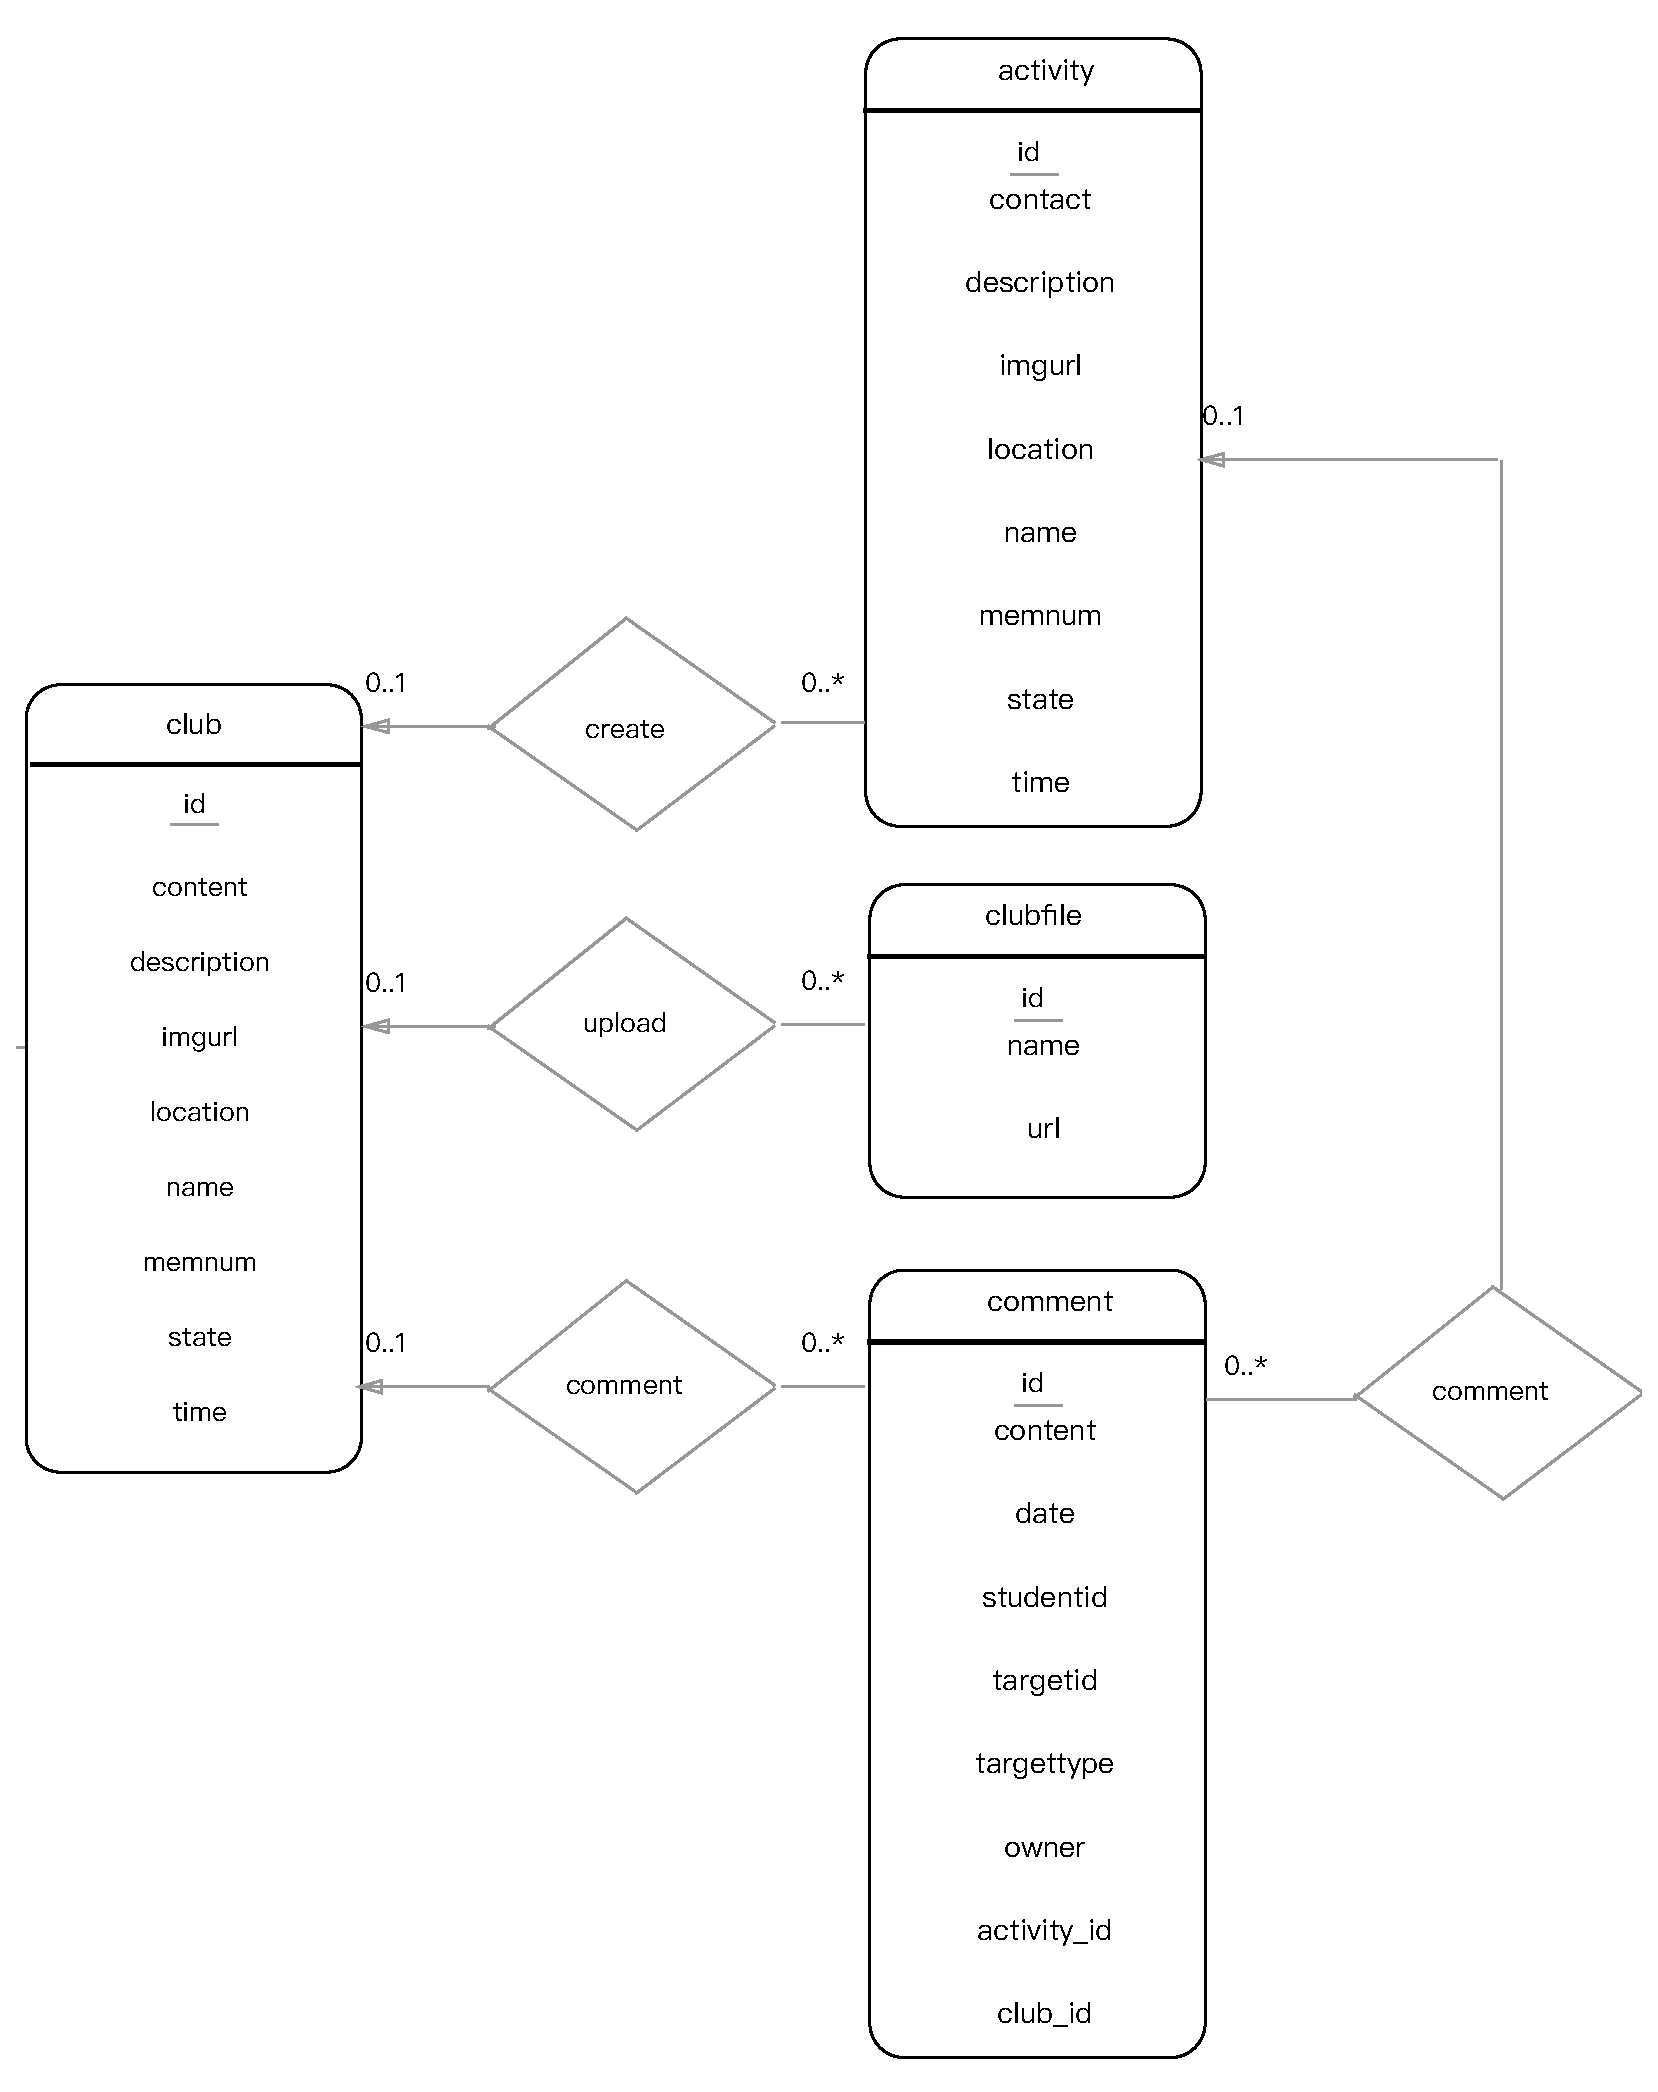
\includegraphics[width = 0.7\textwidth]{club-*-er.eps}
\end{figure}

\subparagraph{comment \& activity}
如下图所示,comment跟activity为一对多的关系,二者以comment关系集相维系,一个activity可以对应有多个comment。
\newline
\begin{figure}[H]
\centering
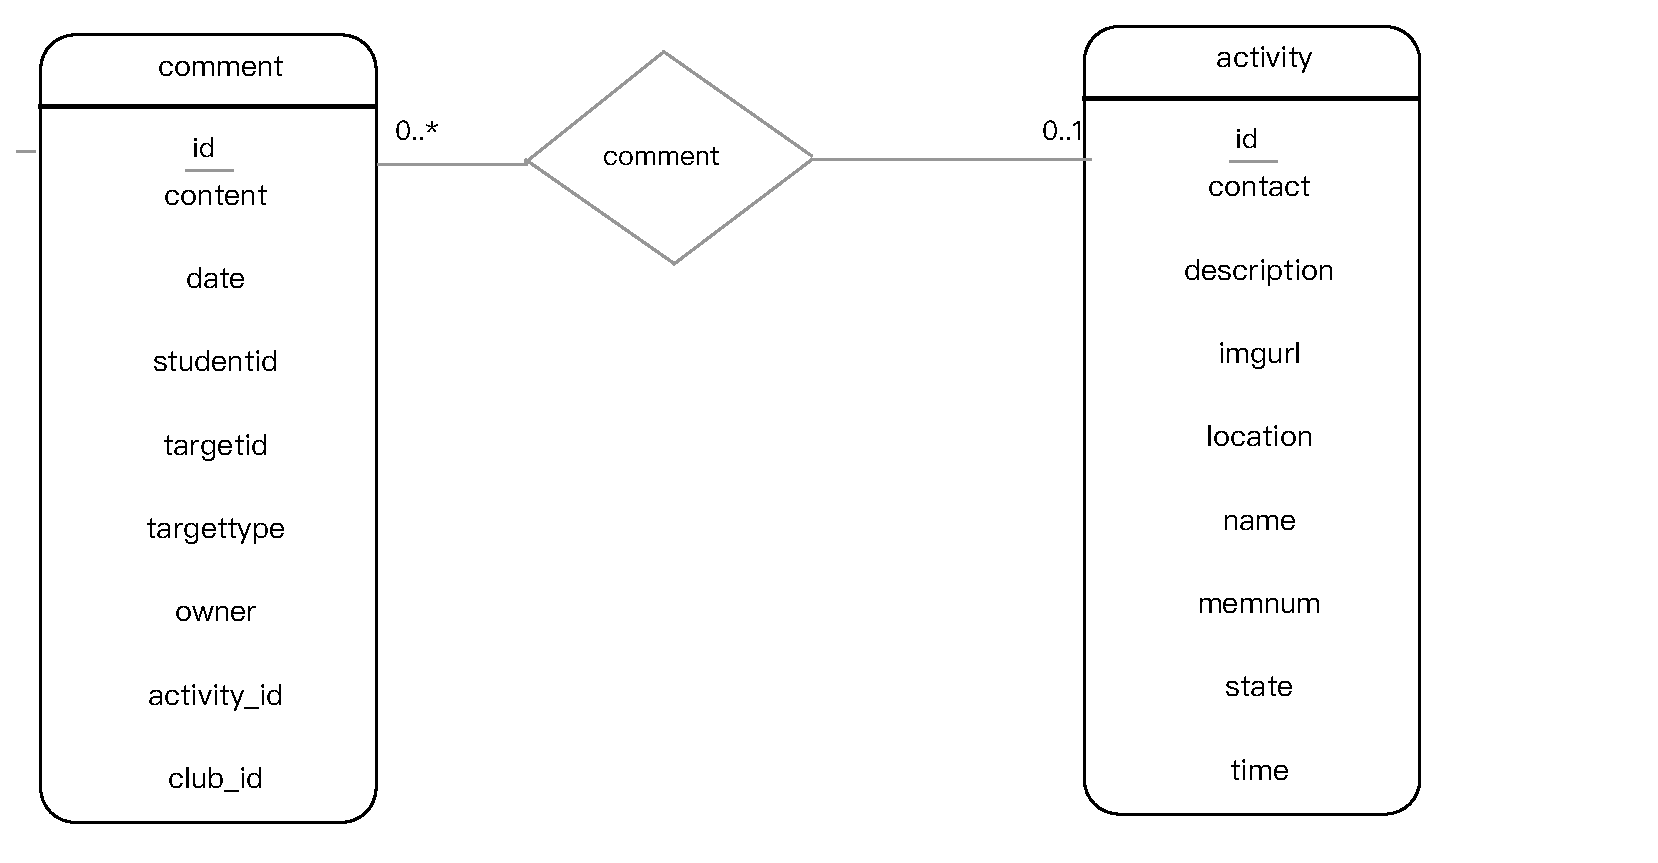
\includegraphics[width = 1.0\textwidth]{activity-comment-er.eps}
\end{figure}

\subparagraph{apply \& club \& teacher}
如下图所示,apply和club、teacher相关联,apply与club为多对一的关系,二者以create apply关系集相维系;apply与teacher为多对一的关系,二者以deal apply关系集相维系,一个teacher可以处理多个apply。
\newline
\begin{figure}[H]
\centering
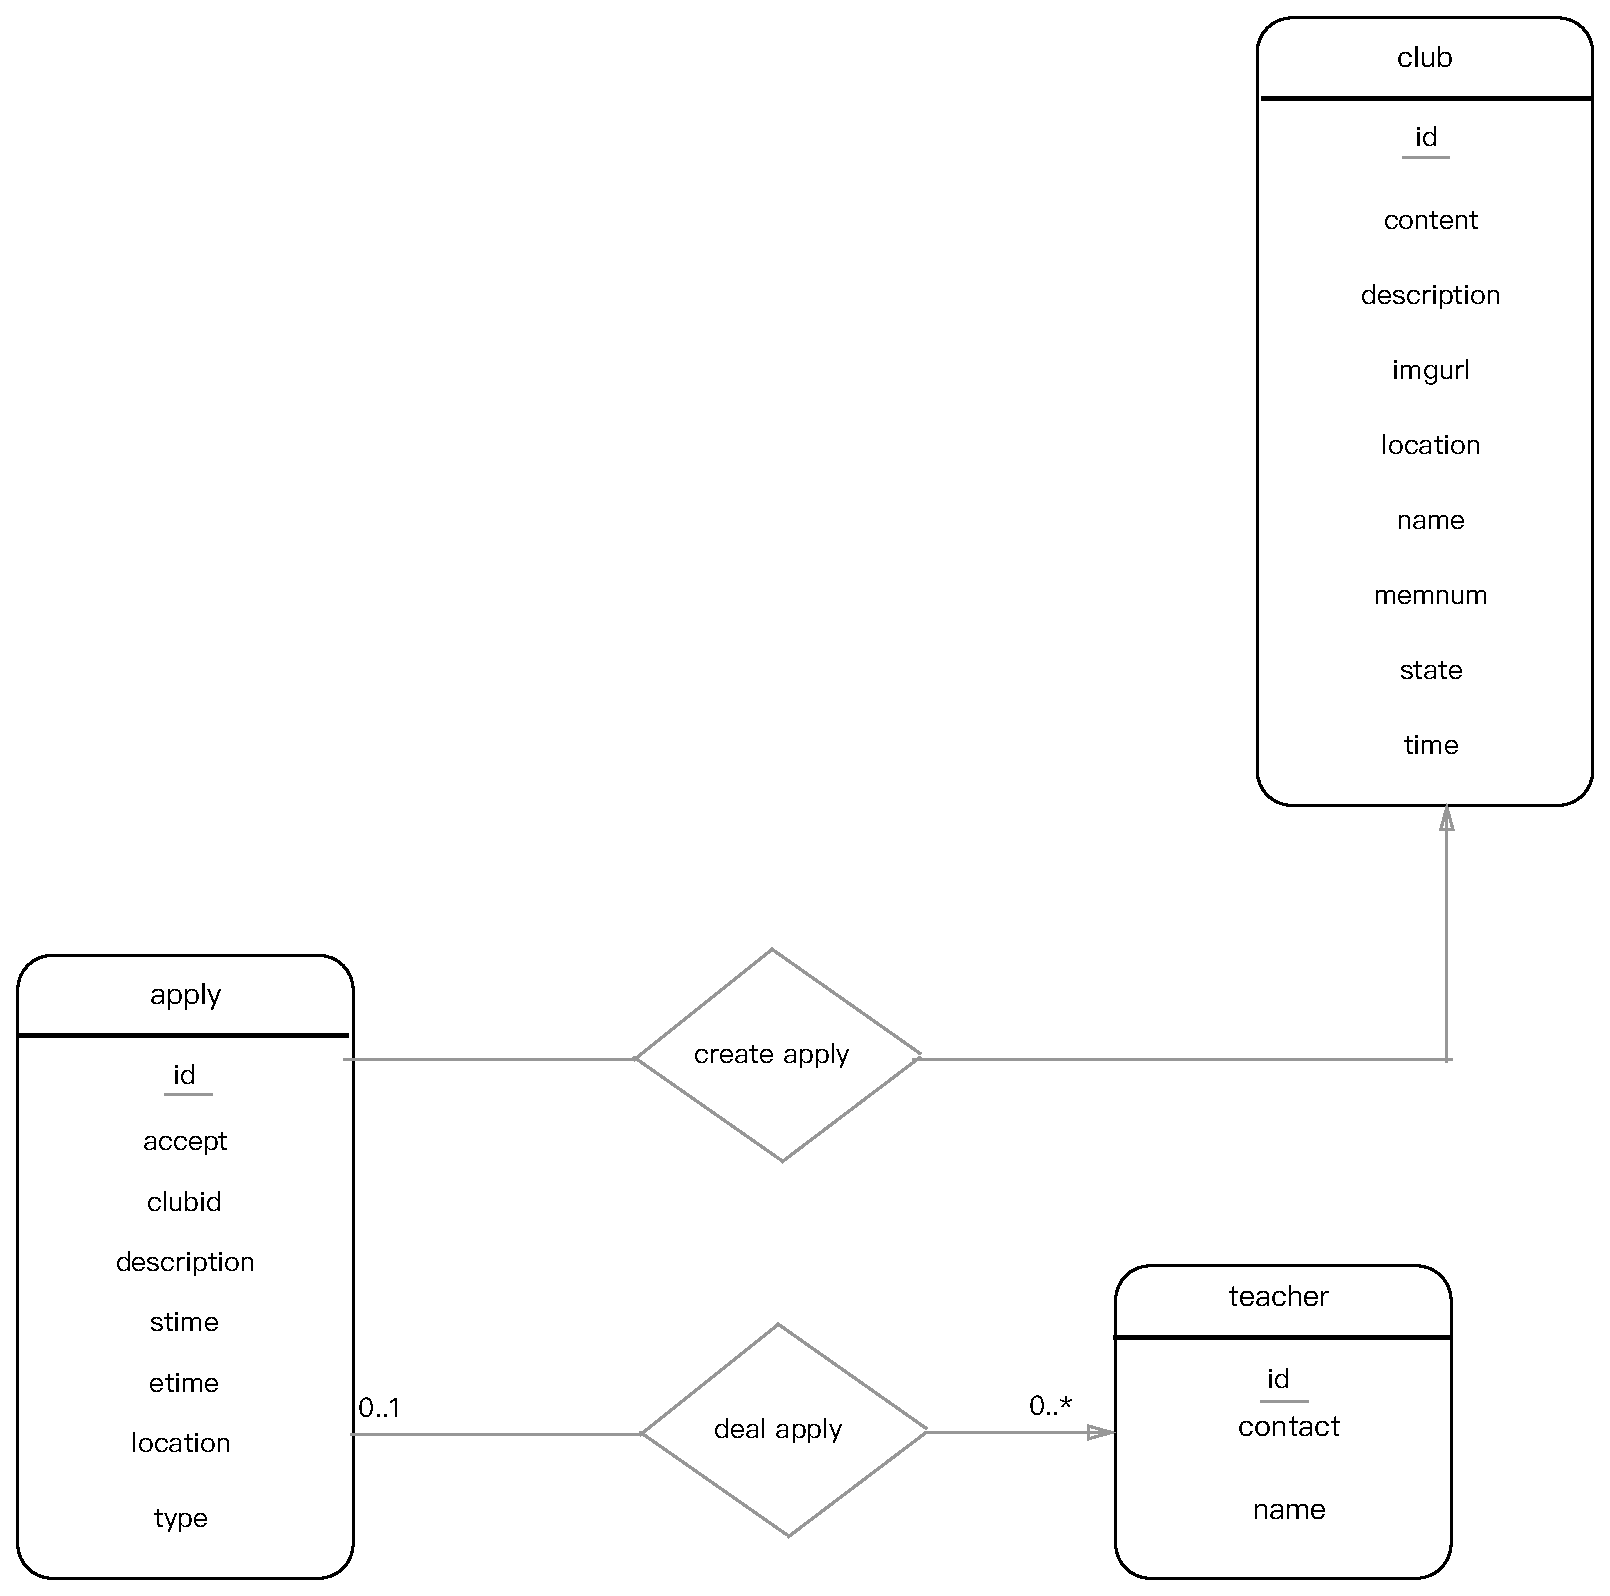
\includegraphics[width = 0.8\textwidth]{apply-*-er.eps}
\end{figure}

\paragraph{实体(Entity)}
本系统中的实体类主要为Student、Teacher、Club、Activity、Apply、Comment、ClubFile:
\begin{figure}[H]
\centering
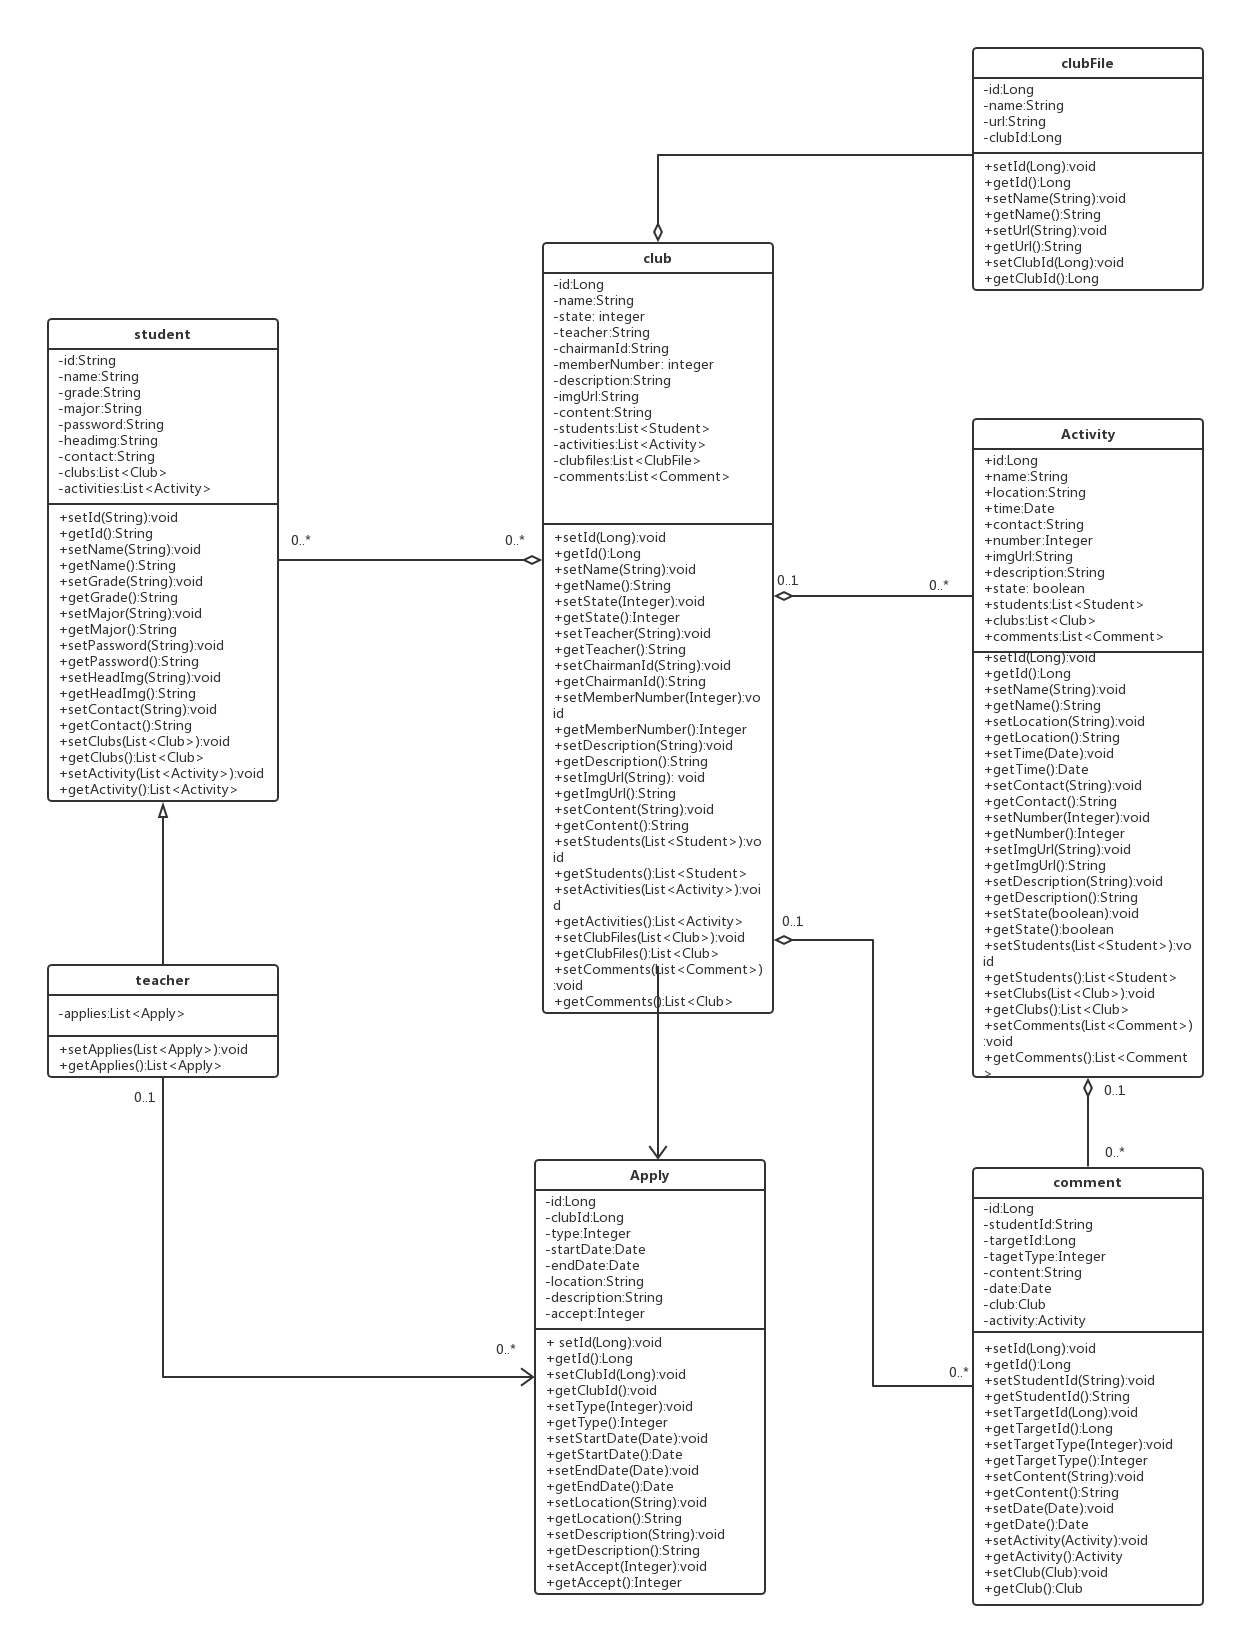
\includegraphics[width = 1.0\textwidth]{xianhuo-class.png}
\end{figure}

\subparagraph{Student}
Student为本系统中普通用户、社团负责人和老师的实体,Teacher继承自Student,具体属性和方法如下图:
\newline
\begin{figure}[H]
\centering
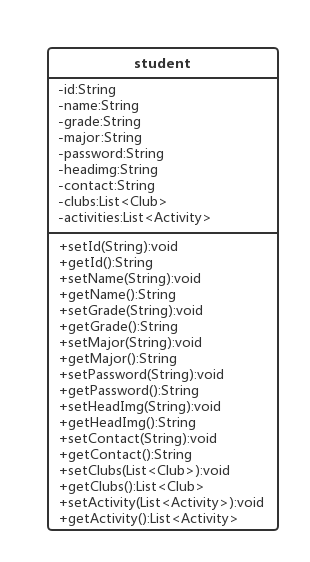
\includegraphics[width = 0.5\textwidth]{student-class.png}
\end{figure}
\begin{table}[H]
\centering
\caption{Student类}
\begin{tabular}{|c|c|c|c|c|c|}
\hline
\multicolumn{6}{|c|}{Student}\\
\hline
类别& 名称& 类型 & 参数 & 返回类型& 备注\\
\hline
\multirow{9}*{属性}
&id & String & 无 & 无 & 学生的学号\\
&name & String & 无 & 无 & 学生的姓名\\
&grade& String & 无 & 无 & 学生的年级\\
&major& String & 无 & 无 & 学生的专业\\
&password& String & 无 & 无 & 学生的密码\\
&headimg& String & 无 & 无 & 学生的头像\\
&contact& String & 无 & 无 & 学生的号码\\
&clubs& List<Club> & 无 & 无 & 学生的参加的社团\\
&activities& List<Activity> & 无 & 无 & 学生参加的活动\\
\hline
\multirow{18}*{方法}
&setId & 无 & String & void & 设置学生的学号\\
&getId & 无 & 无 & String & 得到学生的学号\\
&setName & 无 & String & void & 设置学生的名字\\
&getName & 无 & 无 & String & 得到学生的姓名\\
&setGrade & 无 & String & void & 设置学生的年级\\
&getGrade & 无 & 无 & String & 得到学生的年级\\
&setMajor & 无 & String & void & 设置学生的专业\\
&getMajor & 无 & 无 & String & 得到学生的专业\\
&setPassword & 无 & String & void & 设置学生的密码\\
&getPassword & 无 & 无 & String & 得到学生的密码\\
&setContact & 无 & String & void & 设置学生的联系方式\\
&getContact & 无 & 无 & String & 得到学生的联系方式\\
&setClubs & 无 & List<Club> & void & 设置学生参加的社团\\
&getClubs & 无 & 无 & String & 得到学生的参加的社团\\
&setHeadImg & 无 & String & void & 设置学生的头像\\
&getHeadImg & 无 & 无 & String & 得到学生的头像\\
&setActivities & 无 & List<Activity> & 无 & 设置学生参加的活动\\
&getActivities & 无 & 无 & List<Activity> & 得到学生参加的活动\\
\hline
\end{tabular}
\end{table}

\subparagraph{Teacher}
Teacher是本系统中管理社团创建和场地申请的老师的实体类,它继承自Student,拥有新的属性applies,具体信息如下图:
\newline
\begin{figure}[H]
\centering
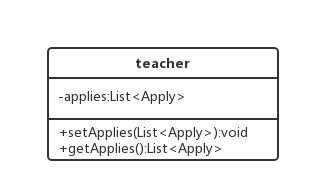
\includegraphics[width = 0.5\textwidth]{teacher-class.png}
\end{figure}
\begin{table}[H]
\centering
\caption{Teacher类}
\begin{tabular}{|c|c|c|c|c|c|}
\hline
\multicolumn{6}{|c|}{Teacher}\\
\hline
类别& 名称& 类型 & 参数 & 返回类型& 备注\\
\hline
\multirow{1}*{属性}
&applies& List<Apply> & 无 & 无 & 老师收到的请求列表\\
\hline
\multirow{2}*{方法}
&setApplies & 无 & List<Apply> & 无 & 设置老师收到的请求\\
&getApplies & 无 & 无 & List<Apply> & 得到老师收到的请求\\
\hline
\end{tabular}
\end{table}

\subparagraph{Activity}
Activity为本系统中社团活动的实体类,具体属性和方法如下图:
\newline
\begin{figure}[H]
\centering
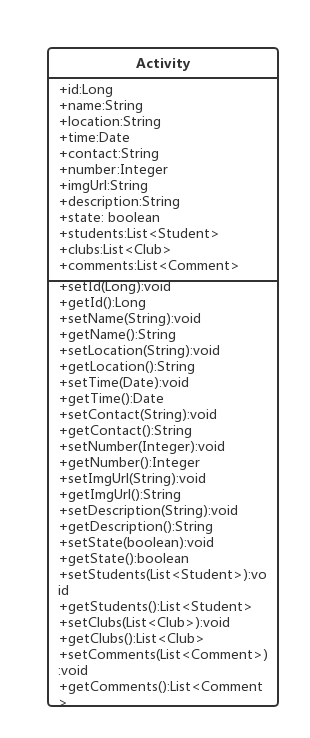
\includegraphics[width = 0.5\textwidth]{activity-class.png}
\end{figure}
\begin{table}[H]
\centering
\caption{Activity类}
\begin{tabular}{|c|c|c|c|c|c|}
\hline
\multicolumn{6}{|c|}{Activity}\\
\hline
类别& 名称& 类型 & 参数 & 返回类型& 备注\\
\hline
\multirow{12}*{属性}
&id & Long & 无 & 无 & 活动的id\\
&name & String & 无 & 无 & 活动的名称\\
&location& String & 无 & 无 & 活动地点\\
&time& Date & 无 & 无 & 活动时间\\
&contact& String & 无 & 无 & 联系方式\\
&number& Integer & 无 & 无 & 参加人数\\
&imgUrl& String & 无 & 无 & 宣传的图片\\
&description& String & 无 & 无 & 活动的描述\\
&state& boolean & 无 & 无 & 活动状态\\
&studentList& List<Student> & 无 & 无 & 参加的学生列表\\
&commentList& List<Comment> & 无 & 无 & 评论列表\\
\hline
\multirow{22}*{方法}
&setId & 无 & Long & void & 设置活动的id\\
&getId & 无 & 无 & Long & 得到活动的id\\
&setName & 无 & String & void & 设置活动的名称\\
&getName & 无 & 无 & String & 得到活动的名称\\
&setLocation & 无 & String & void & 设置活动的地点\\
&getLocation & 无 & 无 & String & 得到活动的地点\\
&setTime & 无 & Date & void & 设置活动的时间\\
&getTime & 无 & 无 & Date & 得到活动的时间\\
&setContact & 无 & String & void & 设置活动的联系方式\\
&getContact & 无 & 无 & String & 得到活动的联系方式\\
&setNumber & 无 & Integer & void & 设置参加活动的人数\\
&getNumber & 无 & 无 & Integer & 得到参加活动的人数\\
&setImgUrl & 无 & String & void & 设置活动的宣传图片\\
&getImgUrl & 无 & 无 & String & 得到活动的宣传图片\\
&setDescription & 无 & String & void & 设置活动的描述\\
&getDescription & 无 & 无 & String & 得到活动的描述\\
&setState & 无 & boolean & void & 设置活动的状态\\
&getState & 无 & 无 & boolean & 得到活动的状态\\
&setStudentList & 无 & List<Student> & void & 设置活动的参加学生\\
&getStudentList & 无 & 无 & List<Student> & 得到活动的参加学生\\
&setCommentList & 无 & List<Comment> & void & 设置活动的评论\\
&getCommentList & 无 & 无 & List<Comment> & 得到活动的评论\\
\hline
\end{tabular}
\end{table}

\subparagraph{Apply}
Apply为本系统中由社团负责人发起的场地申请或海报申请的实体类,具体信息如下:
\newline
\begin{figure}[H]
\centering
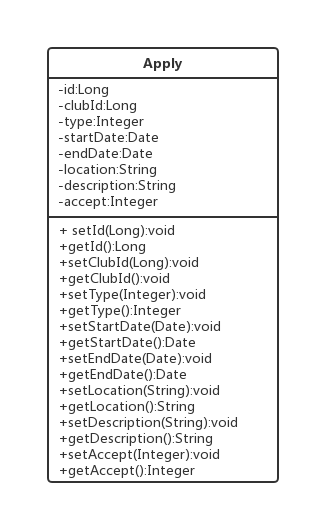
\includegraphics[width = 0.5\textwidth]{apply-class.png}
\end{figure}
\begin{table}[H]
\centering
\caption{Apply类}
\begin{tabular}{|c|c|c|c|c|c|}
\hline
\multicolumn{6}{|c|}{Apply}\\
\hline
类别& 名称& 类型 & 参数 & 返回类型& 备注\\
\hline
\multirow{8}*{属性}
&id & Long & 无 & 无 & 申请的id\\
&clubId & Long & 无 & 无 & 发起申请的社团的id\\
&type& Integer & 无 & 无 & 申请的类型\\
&startDate& Date & 无 & 无 & 申请的开始时间节点\\
&endDate& Date & 无 & 无 & 申请的结束时间节点\\
&location& String & 无 & 无 & 申请的地点\\
&description& String & 无 & 无 & 申请的理由\\
&accept& Integer & 无 & 无 & 申请的状态\\
\hline
\multirow{16}*{方法}
&setId & 无 & Long & void & 设置申请的id\\
&getId & 无 & 无 & Long & 得到申请的id\\
&setClubId & 无 & Long & void & 设置申请的社团的id\\
&getClubId & 无 & 无 & Long & 得到申请的社团的id\\
&setType & 无 & Integer & void & 设置申请的类型\\
&getType & 无 & 无 & Integer & 得到申请的类型\\
&setStartTime & 无 & Date & void & 设置申请的开始的时间节点\\
&getEndTime & 无 & 无 & Date & 得到申请的开始的时间节点\\
&setEndTime & 无 & Date & void & 设置申请的结束的时间节点\\
&getEndTime & 无 & 无 & Date & 得到申请的结束的时间节点\\
&setLocation & 无 & String & void & 设置申请的地点\\
&getLocation & 无 & 无 & String & 得到申请的地点\\
&setDescription & 无 & String & void & 设置申请的理由\\
&getDescription & 无 & 无 & String & 得到申请理由\\
&setAccept & 无 & Integer & void & 设置申请的状态\\
&getAccept & 无 & 无 & Integer & 得到申请的状态\\
\hline
\end{tabular}
\end{table}

\subparagraph{Club}
Club为本系统中的核心类,几乎所有操作都会跟这个实体类有一定的关系,其属性和方法也比较多,具体信息如下:
\newline
\begin{figure}[H]
\centering
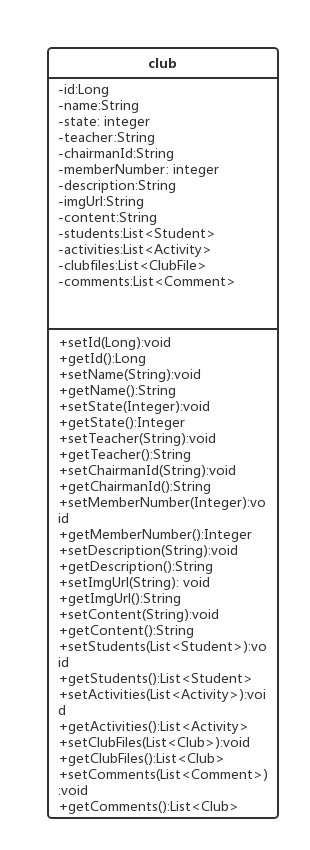
\includegraphics[width = 0.5\textwidth]{club-class.png}
\end{figure}
\begin{table}[H]
\centering
\caption{Club类}
\begin{tabular}{|c|c|c|c|c|c|}
\hline
\multicolumn{6}{|c|}{Club}\\
\hline
类别& 名称& 类型 & 参数 & 返回类型& 备注\\
\hline
\multirow{13}*{属性}
&id & Long & 无 & 无 & 社团的id\\
&name & String & 无 & 无 & 社团的名称\\
&state& Integer & 无 & 无 & 社团的审核状态\\
&teacher& String & 无 & 无 & 社团的指导老师\\
&chairmanId& String & 无 & 无 & 社团主席的id\\
&menberNumber& Integer & 无 & 无 & 社员人数\\
&imgUrl& String & 无 & 无 & 社团的展示封面\\
&description& String & 无 & 无 & 社团的描述\\
&content& String & 无 & 无 & 社团申请标语\\
&students& List<Student> & 无 & 无 & 社员列表\\
&activities& List<Activity> & 无 & 无 & 活动列表\\
&comments& List<Comment> & 无 & 无 & 评论列表\\
&clubFiles& List<clubFile> & 无 & 无 & 资源文件列表\\
\hline
\multirow{26}*{方法}
&setId & 无 & Long & void & 设置社团的id\\
&getId & 无 & 无 & Long & 得到社团的id\\
&setName & 无 & String & void & 设置社团的名称\\
&getName & 无 & 无 & String & 得到社团的名称\\
&setState & 无 & Integer & void & 设置社团的审核状态\\
&getState & 无 & 无 & Integer & 得到社团的审核状态\\
&setTeacher & 无 & String & void & 设置社团的指导老师\\
&getTeacher & 无 & 无 & String & 得到社团的指导老师\\
&setChairManId & 无 & String & void & 设置社团的主席id\\
&getChairManId & 无 & 无 & String & 得到社团的主席id\\
&setContent & 无 & String & void & 设置社团的申请标语\\
&getContent & 无 & 无 & String & 得到社团的申请标语\\
&setMemberNumber & 无 & Integer & void & 设置参加社员的人数\\
&getMenberNumber & 无 & 无 & Integer & 得到参加社员的人数\\
&setImgUrl & 无 & String & void & 设置社团的封面图片\\
&getImgUrl & 无 & 无 & String & 得到社团的封面图片\\
&setDescription & 无 & String & void & 设置社团的描述\\
&getDescription & 无 & 无 & String & 得到社团的描述\\
&setStudents & 无 & List<Student> & void & 设置社员\\
&getStudents & 无 & 无 & List<Student> & 得到社员\\
&setComments & 无 & List<Comment> & void & 设置社团的评论\\
&getComments & 无 & 无 & List<Comment> & 得到社团的评论\\
&setActivities & 无 & List<Activity> & 无 & 设置社团活动\\
&getActivities & 无 & 无 & List<Activity> & 得到社团的活动\\
&setClubFiles & 无 & List<ClubFile> & 无 & 设置社团资源文件\\
&getClubFiles & 无 & 无 & List<ClubFile> & 得到社团资源文件\\
\hline
\end{tabular}
\end{table}

\subparagraph{Comment}
Comment为本系统中评论的实体类,由Student创建,跟Club和Activity相关联,具体信息如下:
\newline
\begin{figure}[H]
\centering
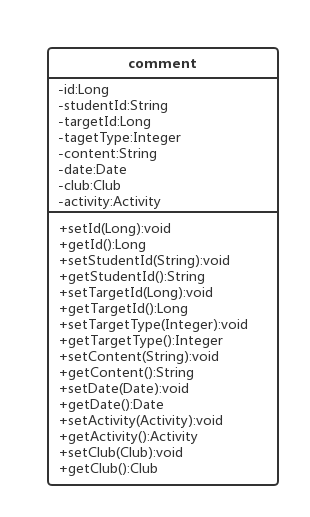
\includegraphics[width = 0.5\textwidth]{comment-class.png}
\end{figure}
\begin{table}[H]
\centering
\caption{Comment类}
\begin{tabular}{|c|c|c|c|c|c|}
\hline
\multicolumn{6}{|c|}{Comment}\\
\hline
类别& 名称& 类型 & 参数 & 返回类型& 备注\\
\hline
\multirow{8}*{属性}
&id & Long & 无 & 无 & 评论的id\\
&studentId & String & 无 & 无 & 发起评论学生的id\\
&targetId& Long & 无 & 无 & 评论目标的id\\
&targetType& Integer & 无 & 无 & 评论目标的类别\\
&content& String & 无 & 无 & 评论的内容\\
&activity& Activity & 无 & 无 & 评论的活动\\
&club& Club & 无 & 无 & 评论的社团\\
&date& Date & 无 & 无 & 评论的时间\\
\hline
\multirow{16}*{方法}
&setId & 无 & Long & void & 设置评论的id\\
&getId & 无 & 无 & Long & 得到评论的id\\
&setStudentId & 无 & String & void & 设置评论学生的id\\
&getStudentId & 无 & 无 & String & 得到评论学生的id\\
&setTargetId & 无 & Long & void & 设置评论目标的id\\
&getTargetId & 无 & 无 & Long & 得到评论目标的id\\
&setTargetType & 无 & Integer & void & 设置评论目标的类别\\
&getTargetType & 无 & 无 & Integet & 得到评论目标的类别\\
&setContent & 无 & String & void & 设置评论内容\\
&getContent & 无 & 无 & String & 得到评论内容\\
&setActivity & 无 & Activity & 无 & 设置评论的活动\\
&getActivity & 无 & 无 & Activity & 得到评论的活动\\
&setClub & 无 & Club & 无 & 设置评论的社团\\
&getClub & 无 & 无 & Club & 得到评论的社团\\
\hline
\end{tabular}
\end{table}

\subparagraph{ClubFile}
ClubFile为本系统中社团资源文件的实体类,由Club创建,由七牛云托管,具体信息如下:
\newline
\begin{figure}[H]
\centering
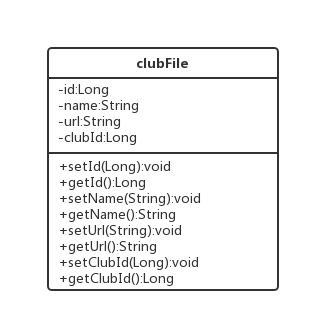
\includegraphics[width = 0.5\textwidth]{clubfile-class.png}
\end{figure}
\begin{table}[H]
\centering
\caption{ClubFile类}
\begin{tabular}{|c|c|c|c|c|c|}
\hline
\multicolumn{6}{|c|}{ClubFile}\\
\hline
类别& 名称& 类型 & 参数 & 返回类型& 备注\\
\hline
\multirow{4}*{属性}
&id & Long & 无 & 无 & 资源文件的id\\
&name & String & 无 & 无 & 资源文件的名称\\
&url& String & 无 & 无 & 资源文件的下载地址\\
&clubId& Long & 无 & 无 & 对应社团的id\\
\hline
\multirow{8}*{方法}
&setId & 无 & Long & void & 设置资源文件的id\\
&getId & 无 & 无 & Long & 得到资源文件的id\\
&setName & 无 & String & void & 设置资源文件的名称\\
&getName & 无 & 无 & String & 得到资源文件的名称\\
&setUrl & 无 & String & void & 设置资源文件的下载地址\\
&getUrl & 无 & 无 & String & 得到资源文件的下载地址\\
&setClubId & 无 & Long & void & 设置对应社团的id\\
&getClubId & 无 & 无 & Long & 得到对应社团的id\\
\hline
\end{tabular}
\end{table}

\paragraph{仓库类和服务类(repository \& Service)}
仓库类和服务类是本项目中不可或缺的一部分,它们管理着实例,为上层的controller提供数据支持,其类图如下:
\newline
\begin{figure}[H]
\centering
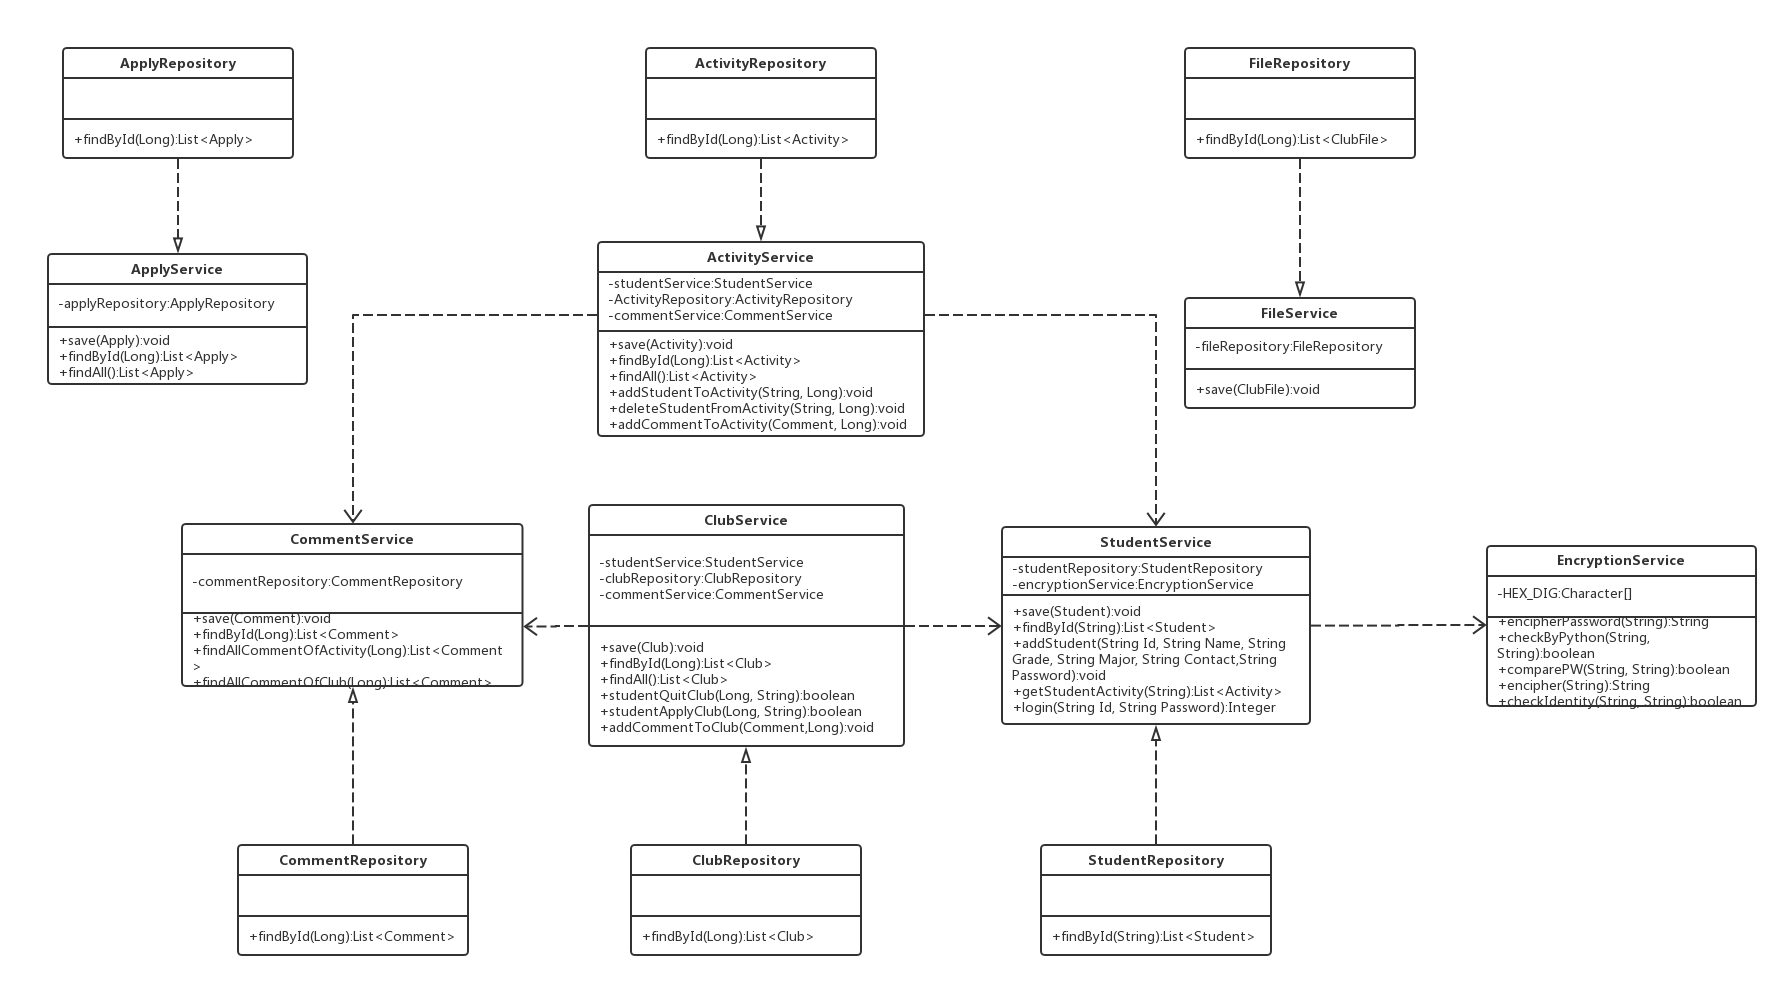
\includegraphics[width = 1.1\textwidth]{repository-service.png}
\end{figure}

\subparagraph{StudentRepository \& StudentService}
StudentRepository和StudentService在本系统中担任管理学生业务的重任,对实体类Student进行一层封装,使其增删改查变的非常容易,以下为其具体细节,因为StudentService为StudentRepository的实现,所以具体介绍StudentService:
\newline
\begin{figure}[H]
\centering
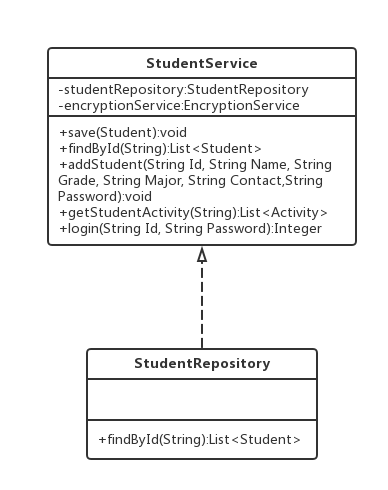
\includegraphics[width = 0.4\textwidth]{student-rs.png}
\end{figure}
\begin{center}
\emph{save(Student student):void}\\
修改数据库中学生信息\\ 
\emph{findById(String Id):List<Student>}\\
根据学生id在数据库中查找学生\\
\emph{addStudent(String Id, String Name, String Grade, String Major, String Contact, String Password):void}\\
根据学生完整信息生成学生存入数据库\\
\emph{getStudentActivity(String Id):List<Activity>}\\
根据学生学号查到某学生并获得他所有的活动\\
\emph{login(String Id, String Password):Integer}\\
对某学生执行登录操作
\end{center}

\subparagraph{ClubRepository \& ClubService}
ClubRepository和ClubService在本系统中担任管理社团业务的重任,对实体类Club进行一层封装,使其增删改查变得非常容易,以下为具体细节,因为ClubService为ClubRepository的实现,所以具体介绍ClubService:
\newline
\begin{figure}[H]
\centering
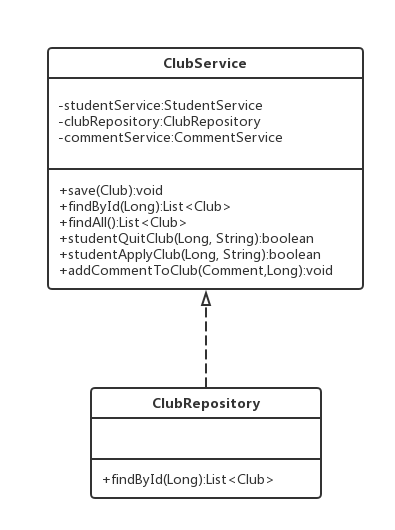
\includegraphics[width = 0.4\textwidth]{club-rs.png}
\end{figure}
\begin{center}
\emph{save(Club club):void}\\
修改数据库中社团的信息\\
\emph{findById(Long Id):List<Club>}\\
根据社团的id查找到社团\\
\emph{findAll():List<Club>}\\
将所有的社团信息返回\\
\emph{studentQuitClub(Long id, String id):boolean}\\
将一个学生退出社团\\
\emph{studentApplyClub(Long id, String id):boolean}\\
学生申请加入社团\\
\emph{addCommentToClub(Comment comment, Long id):void}\\
对俱乐部进行评论\\
\end{center}

\subparagraph{ActivityRepository \& ActivityService}
ActivityRepository和ActivityService在本系统中担任管理活动业务的重任,对实体类Activity进行一层封装,使其增删改查变得非常容易,以下为具体细节,因为ActivityService为ActivityRepository的实现,所以具体介绍ActivityService:
\newline
\begin{figure}[H]
\centering
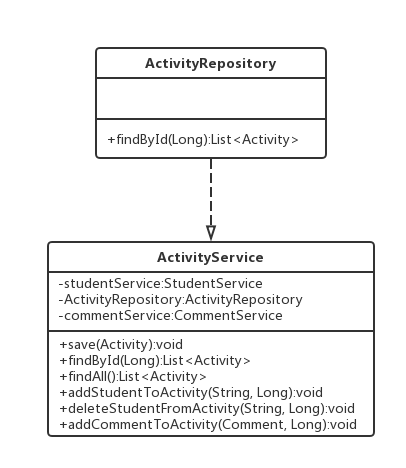
\includegraphics[width = 0.4\textwidth]{activity-rs.png}
\end{figure}
\begin{center}
\emph{save(Activity activity):void}\\
修改数据库中活动的信息\\
\emph{findById(Long Id):List<Activity>}\\
根据活动的id查找到活动\\
\emph{findAll():List<Activity>}\\
将所有的活动信息返回\\
\emph{addStudentToActivity(String id, Long id):void}\\
将一个学生加入一个活动中\\
\emph{deleteStudentFromActivity(String id, Long id):void}\\
将一个学生从一个活动中删除\\
\emph{addCommentToActivity(Comment comment, Long id):void}\\
对活动进行评论
\end{center}

\subparagraph{ApplyRepository \& ApplyService}
ApplyRepository和ApplyService在本系统中担任管理请求业务的重任,对实体类Apply进行一层封装,使其增删改查变得非常容易,以下为具体细节,因为ApplyService为ApplyRepository的实现,所以具体介绍ApplyService:
\newline
\begin{figure}[H]
\centering
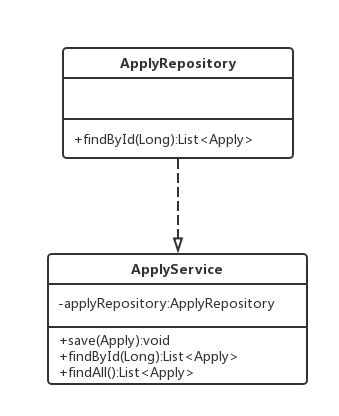
\includegraphics[width = 0.4\textwidth]{apply-rs.png}
\end{figure}
\begin{center}
\emph{save(Apply apply):void}\\
修改数据库中请求的信息\\
\emph{findById(Long Id):List<Apply>}\\
根据请求的Id查找到请求\\
\emph{findAll():List<Apply>}\\
返回全部请求
\end{center}

\subparagraph{CommentRepository \& CommentService}
CommentRepository和CommentService在本系统中担任管理评论业务的重任,对实体类Comment进行一层封装,使其增删改查变得非常容易,以下为具体细节,因为CommentService为CommentRepository的实现,所以具体介绍CommentService:
\newline
\begin{figure}[H]
\centering
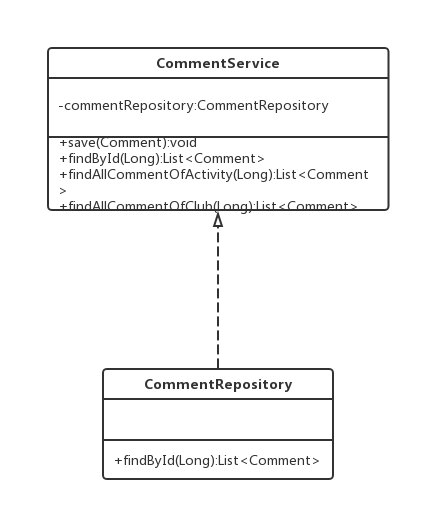
\includegraphics[width = 0.4\textwidth]{comment-rs.png}
\end{figure}
\begin{center}
\emph{save(Comment comment):void}\\
修改数据库中评论的信息\\
\emph{findById(Long Id):List<Comment>}\\
根据请求的Id查找到评论\\
\emph{findAllCommentOfClub(Long Id):List<Comment>}\\
返回某个社团的所有评论\\
\emph{findAllCommentOfActivity(Long Id):List<Comment>}\\
返回某个活动的所有评论
\end{center}

\subparagraph{FileRepository \& FileService}
ClubFileRepository和ClubFileService在本系统中担任管理社团资源文件业务的重任,对实体类ClubFile进行一层封装,使其增删改查变得非常容易,以下为具体细节,因为ClubFileService为ClubFileRepository的实现,所以具体介绍ClubFileService:
\newline
\begin{figure}[H]
\centering
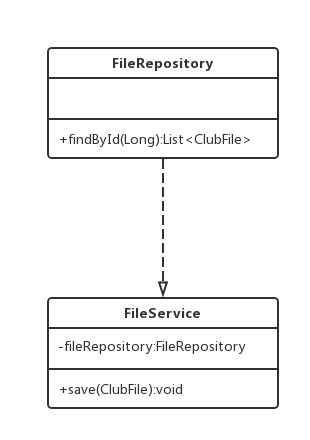
\includegraphics[width = 0.4\textwidth]{clubfile-rs.png}
\end{figure}
\begin{center}
\emph{save(ClubFile clubFile):void}\\
修改数据库中俱乐部资源文件的信息
\end{center}

\subparagraph{EncryptionService}
EncryptionService为学生的登录提供MD5加密服务,在每次登录的时候这个服务类都会把明文密码转化为用MD5加密的密文,以下为具体细节:
\newline
\begin{figure}[H]
\centering
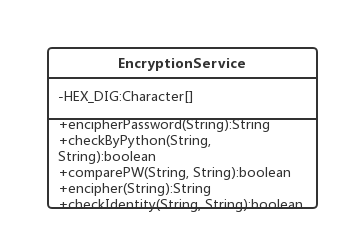
\includegraphics[width = 0.4\textwidth]{Encryption-rs.png}
\end{figure}
\begin{center}
\emph{encipherPassword(String Password):String}\\
将给定的明文密码转化为MD5密文\\
\emph{checkByPython(String Id, String Password):boolean}\\
使用python脚本访问4m3本研一体化网站验证账号\\
\emph{comparePW(String Id, String Password):boolean}\\
比对用户的账号和密码是不是和数据库中的吻合\\
\emph{encipher(String Password):String}\\
对密文进行撒盐\\
\emph{checkIdentity(String Id, String Password):boolean}\\
验明身份并写session
\end{center}

\subsubsection{行为建模}
张

\section{UI 需求}
洪

\section{非功能需求}
\subsection{性能需求}
洪
\subsubsection{精度}

\subsubsection{时间特性要求}

\subsubsection{输入输出要求}

\subsection{数据管理能力要求}
张
\subsection{安全及保密性要求}
张
\subsection{灵活性要求}
夏
\subsection{其他专门要求}
夏
\section{运行环境规定}
\subsection{设备}

\subsection{支持软件}
张
\section{需求跟踪}
夏
\section{附录}

\end{document}
